\documentclass[12pt]{article}
\usepackage[main=russian, english]{babel}
\usepackage[utf8]{inputenc}
\usepackage{amsmath}
\usepackage{booktabs}
\usepackage{float}
\usepackage{geometry}
\usepackage{parskip}
\usepackage{pgf}
\usepackage{siunitx}

\geometry{
    a4paper,
    left=20mm,
    right=20mm,
    top=20mm,
}

\title{Отчет по лабораторной работе "Исследование спектра $\beta$-частиц"}
\date{}

\begin{document}
\maketitle

\section{Цель работы}
С помощью магнитного спектрометра пронаблюдать энергетический спектр
$\beta$-частиц при распаде ядер $^{137}$Cs
и определить их максимальную энергию.

\section{Теоретические сведения}

$\beta$-распад описывается формулой:
\begin{equation*}
    ^A_Z \text{X} = ^A_{Z+1} \text{X} + e^- + \tilde{\nu}
\end{equation*}

Большая часть энергии реакции распределена между электроном и антинейтрино, поэтому:
\begin{equation*}
    T_{max} = T + E_{\tilde{\nu}}
\end{equation*}

Плотность вероятности для импульса электрона:
\begin{gather*}
    W(p) \propto p^2 p_{\tilde{\nu}}^2 \\
    p_{\tilde{\nu}} = \frac{E_{\tilde{\nu}}}{c} = \frac{T_{max} - T}{c} \\
    W(p) \propto p^2 \left( T_{max} - T \right)^2 \\
\end{gather*}

Кинетическая энергия электрона:
\begin{gather*}
    T = \sqrt{p^2 c^2 - m_e^2 c^4} - m_e c^2
\end{gather*}

Часть из образовавшихся в результате $\beta$-распада ядер находятся в возбужденном состоянии.
Поэтому они либо излучают $\gamma$-квант, либо электрон с электрон с внешней оболочки.
Таких электроны называются конверсионными и обладают строго фиксированная энергий \input{Tconv}.

\begin{figure}[h!]
    \caption{Плотность распределения с учетом конверсионных электронов}
    \centering
    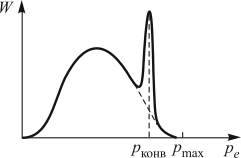
\includegraphics[width=0.5\linewidth]{dist.png}
\end{figure}

\section{Экспериментальная установка}

\begin{figure}[H]
    \caption{Магнитный спектрометр}
    \centering
    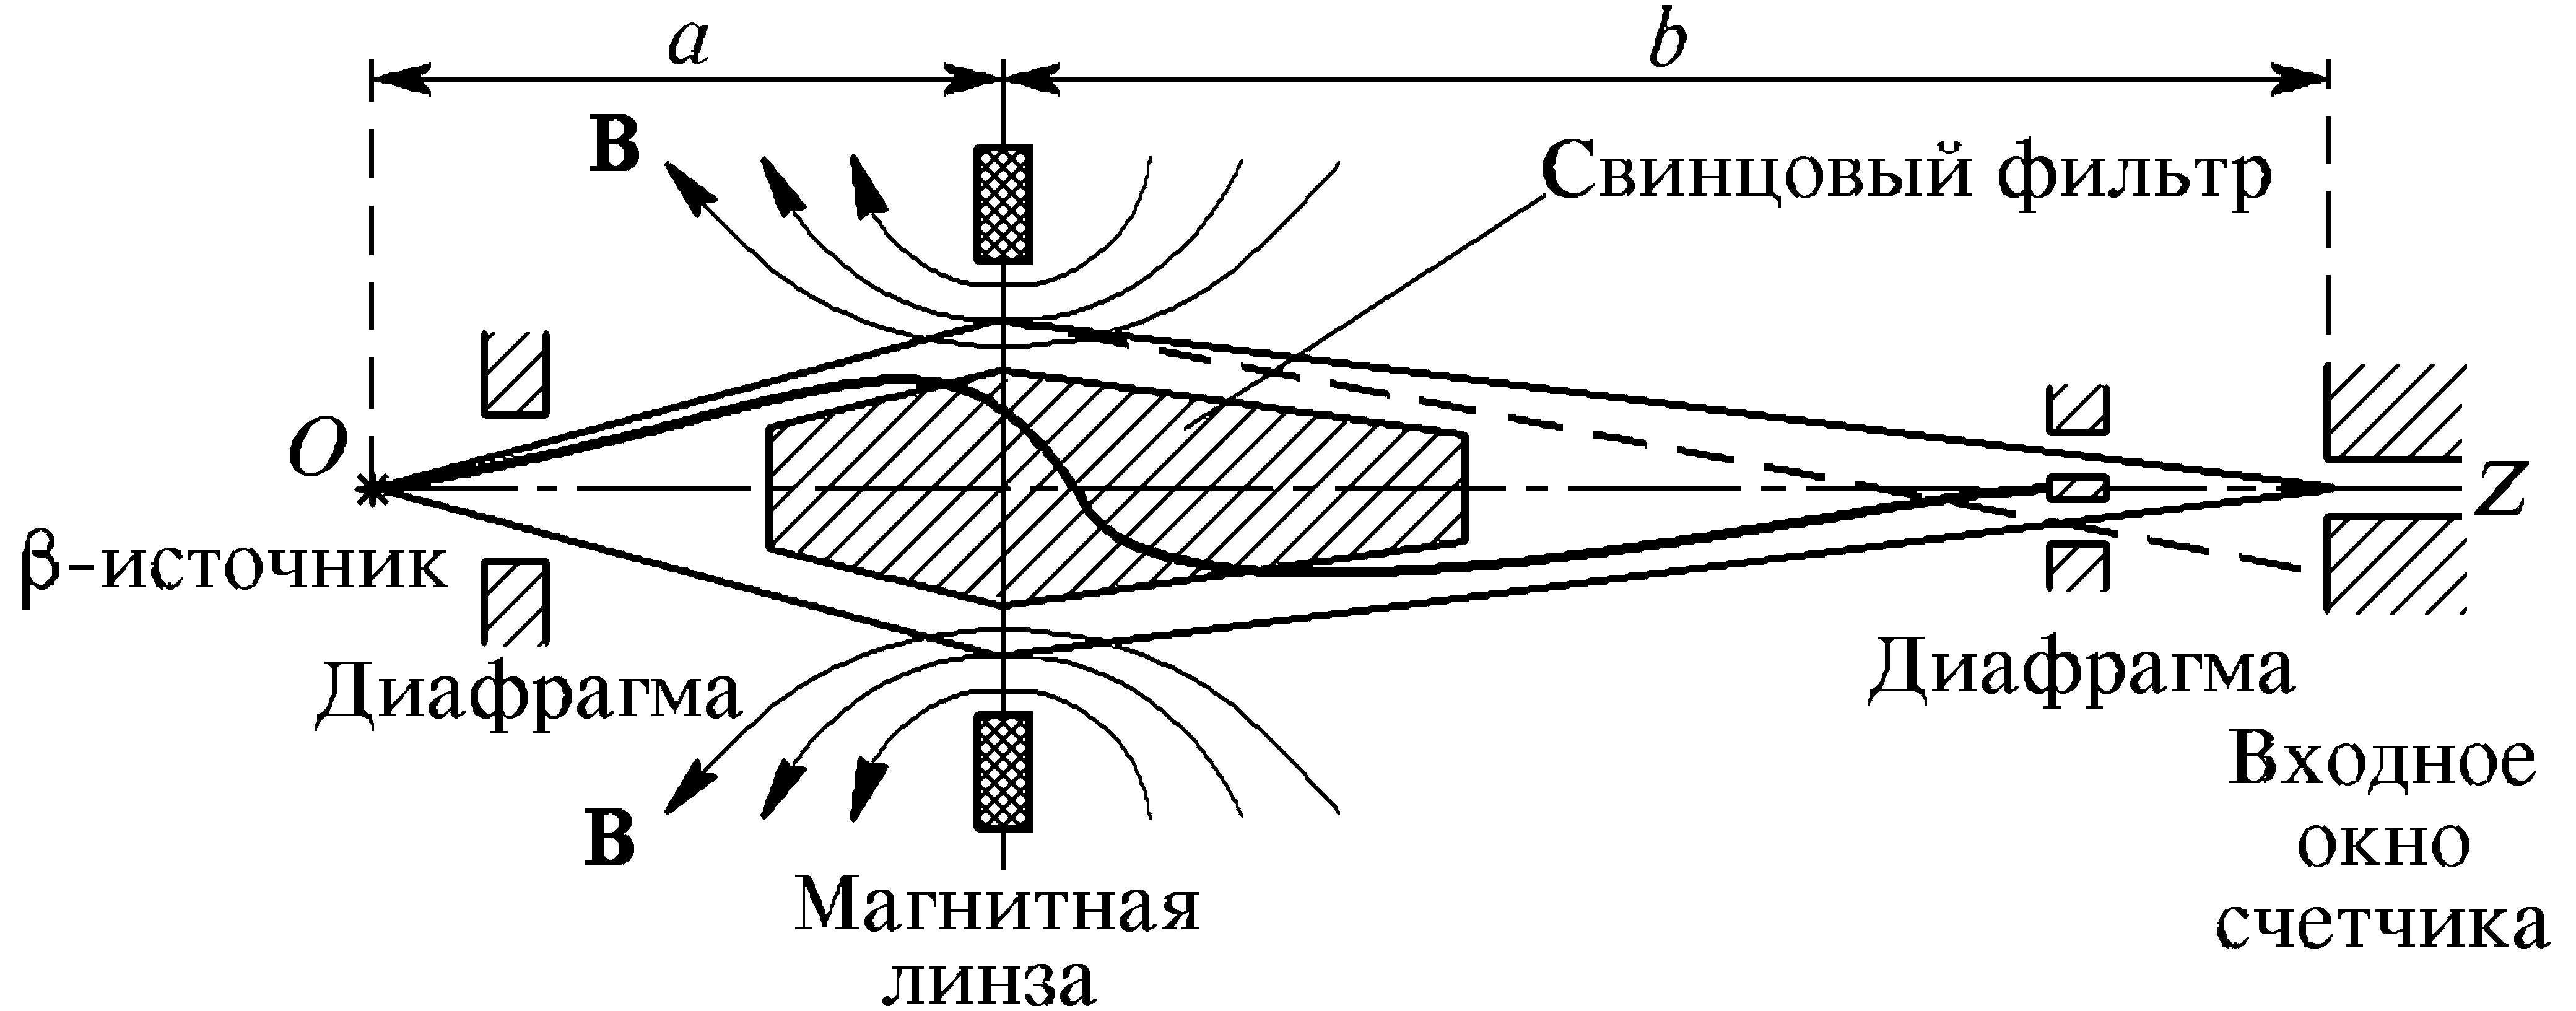
\includegraphics[width=\linewidth]{dev.png}
\end{figure}

Фокусное расстояние катушки зависит от тока и импульса электронов:
\begin{gather*}
    \frac{1}{f} \propto \frac{I^2}{p^2}
\end{gather*}

Изменяя ток через катушку, можно фокусировать электроны с разными значениями
импульса на счетчике.
Таким образом, импульс зарегистрированных электронов пропорционален току через катушку:
\begin{gather*}
    p = kI
\end{gather*}

Количество зарегистрированных электронов зависит от разрешающей способности спектрометра:
\begin{gather*}
    N(p) = W(p) \Delta p
\end{gather*}

Найдем эту разрешающую способность:
\begin{gather*}
    f = C \frac{p^2}{I^2} \\ 
    \Delta f = C \frac{2 p \Delta p}{I^2} \\ 
    \Delta p =
        \Delta f \frac{I^2} {2 p C} =
        \frac{1}{2} \frac{\Delta f}{f} p \\
\end{gather*}

Смысл $\Delta f$ - максимальное различие между $f$
и фокусным расстоянием для электрона, при котором счетчик еще учтет его.
Этот параметр геометрии установки, и следовательно никак не зависит от тока через катушку.

Находим связь между количеством зарегистрированных электронов и плотностью вероятности:
\begin{gather*}
    N(p) \propto W(p) p
\end{gather*}

\section{Результаты измерений}

\begin{table}[H]
\begin{center}
\input{data.tab.tex}
\end{center}
\end{table}

Уровень фона:
\input{noise}

Построим график $N(I)$ с учетом фона:

\begin{figure}[H]
    \centering
    \input{data.pgf}
\end{figure}

Здесь мы видим какой-то третий пик, наличие которого теория не предполагает.

Найдем по графику и таблице положение конверсионного пика и определим по нему $k$:
\input{conv}

\begin{table}[H]
\begin{center}
\input{data2.tab.tex}
\end{center}
\end{table}

Построим графики $N(p)$ и $N(T)$. Не будем учитывать точки, где $N < 0$:

\begin{figure}[H]
    \centering
    \input{data2.pgf}
\end{figure}

\begin{figure}[H]
    \centering
    \input{data3.pgf}
\end{figure}

Построим график Ферми:

\begin{figure}[H]
    \centering
    \input{fermi.pgf}
\end{figure}

По графику видно, что на участке $T \in [240; 600]$ зависимость линейна:
\input{Tmax}

Табличное значение энергии распада для ${^{137}}$Cs ${T_{max}}_{ref}= \qty[]{512}{keV}$.

\section{Заключение}
Был изучен спектр энергий электронов при $\beta$-распаде ${^{137}}$Cs и найдена энергия этого процесса.
Однако полученный результат не соответствует табличному.

\end{document}
